% Copyright (c) 2017 Aleksa Sarai <asarai@suse.de>
% This work is licensed under the Creative Commons Attribution-ShareAlike 4.0
% International License. To view a copy of this license, visit
% http://creativecommons.org/licenses/by-sa/4.0/ or send a letter to Creative
% Commons, PO Box 1866, Mountain View, CA 94042, USA.

\documentclass[10pt,aspectratio=169]{beamer}
\usetheme{metropolis}
\metroset{background=light}
\metroset{titleformat=smallcaps}

\usepackage{pbox}
\usepackage{fontspec}
\usepackage[absolute,overlay]{textpos}
\usepackage[math-style=TeX]{unicode-math}
\usepackage{booktabs}

\usepackage{tikz}
\usetikzlibrary{calc}

\usepackage{hyperref}
\usepackage{graphicx}
\graphicspath{{.}{assets/}}

\setbeamertemplate{caption}{\raggedright\insertcaption\par}

\title{Rootless Containers with \texttt{runc}}
\author{%
		Aleksa Sarai \\
		Software Engineer \\
		SUSE \\
		\href{mailto:asarai@suse.de}{\tiny\tt \underline{asarai@suse.de}}}

\date{}
\institute{}

\begin{document}
	\begin{frame}[plain,noframenumbering]
		\begin{tikzpicture}[remember picture,overlay]
			\node[anchor=north east] at ($(current page.north east) - (-0.3, 0.3)$) {
\includegraphics[height=2cm]{man-in-business-suit-levitating}};
			\node[anchor=south east] at ($(current page.south east) + (-0.3, 0.3)$) {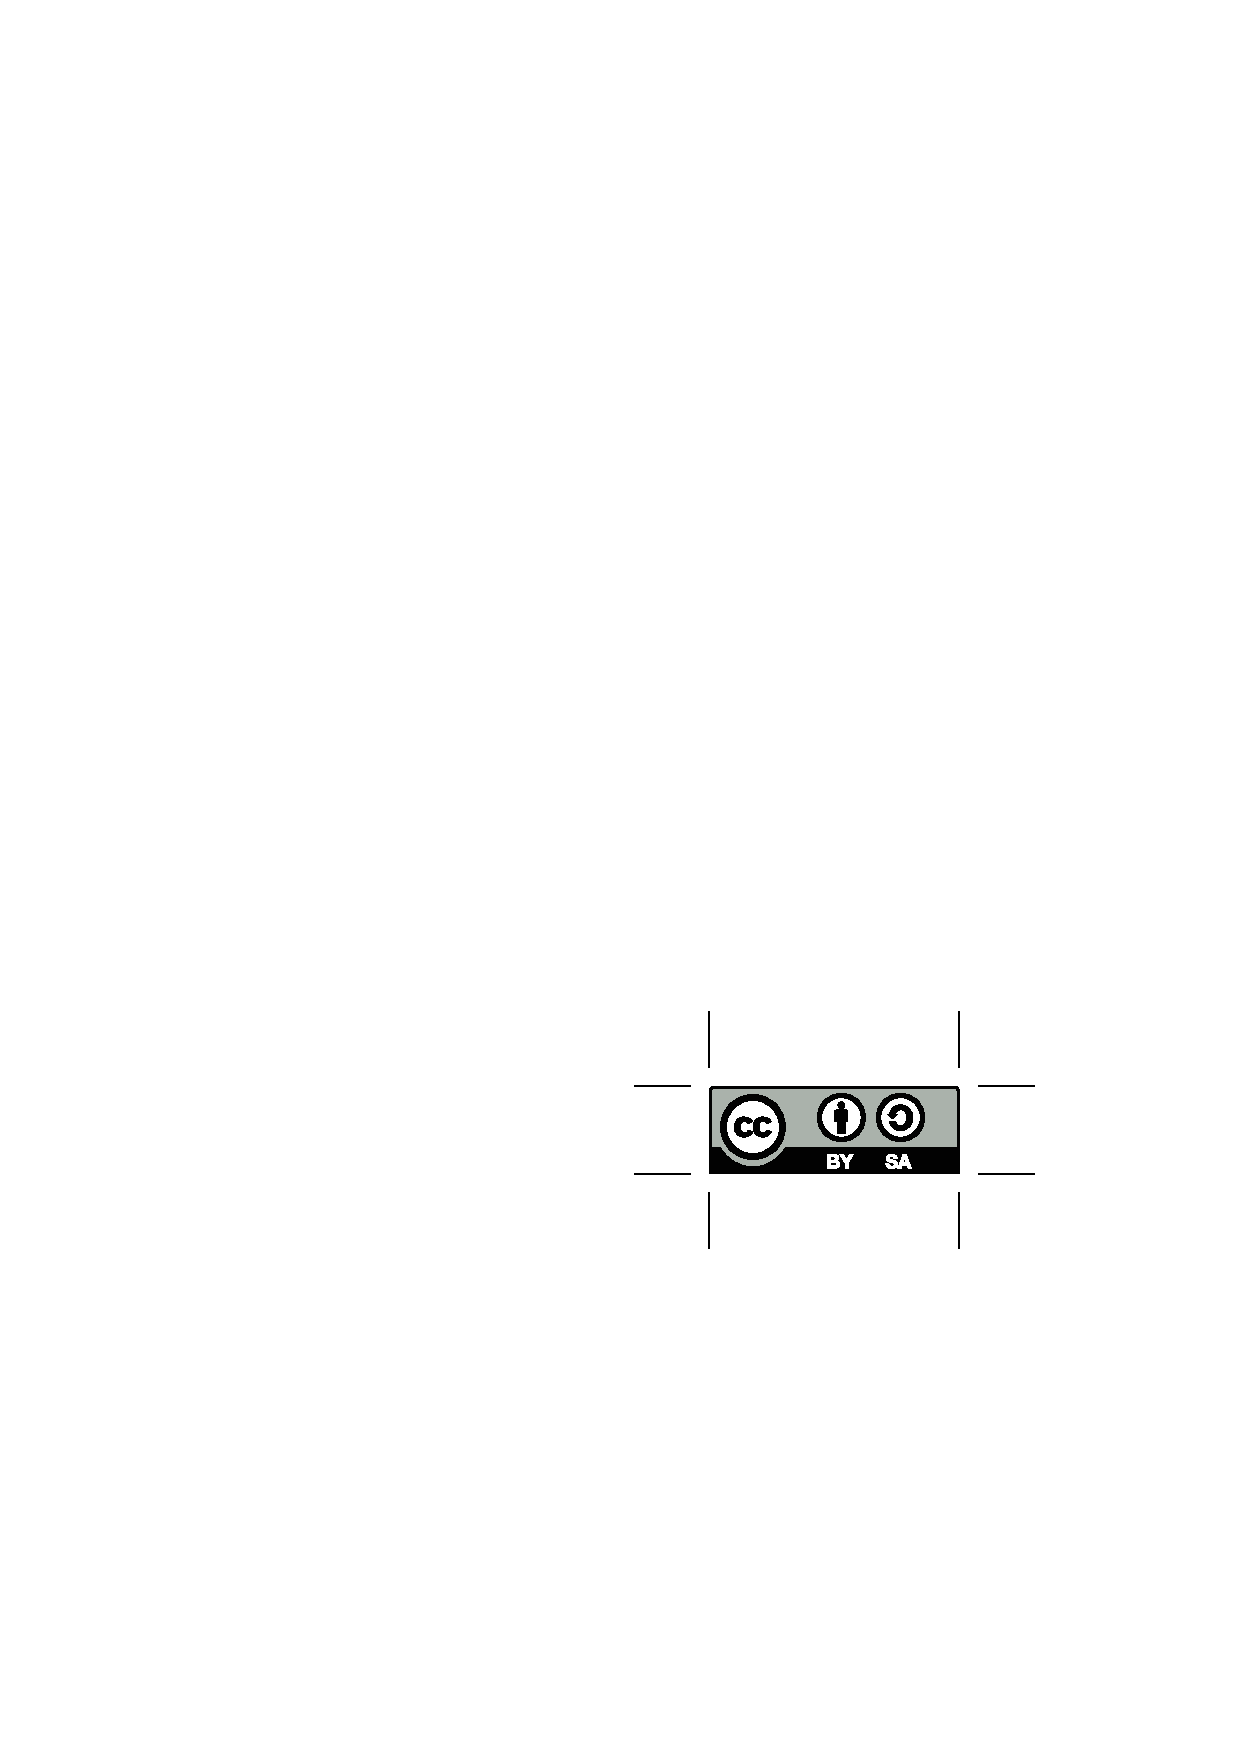
\includegraphics[width=1.6cm]{cc_by_sa}};
			\node[anchor=south east] at ($(current page.south east) + (-0.13, 0.8)$) {
\includegraphics[width=2cm]{talk_qr}};
			\node[anchor=south west] at ($(current page.south west) + (2.3, 0.3)$) {
\includegraphics[height=0.6cm]{oci_logo}};
			\node[anchor=south west] at ($(current page.south west) + (0.3, 0.3)$) {
\includegraphics[height=0.75cm]{suse_logo}};
		\end{tikzpicture}

		\titlepage%
	\end{frame}

	\begin{frame}{``Required Reading''}
	    \begin{itemize}
	        \item ``Kubernetes meets Linux'' --- \textbf{Vishnu Kannan} --- $1030$ yesterday.
	        \item ``Containers from scratch - the sequel!'' --- \textbf{Liz Rice} --- $1235$ yesterday.
	        \item ``OCI and Open Container Standards'' --- \textbf{Jonathan Boulle} --- $1645$ yesterday.
	        \item ``Mixing cgroupfs v1 and cgroupfs v2'' --- \textbf{Christian Brauner} --- T-plus $35$ minutes.
	    \end{itemize}
	\end{frame}

	\begin{frame}{\textit{Revision}: Open Container Initiative}
		\begin{itemize}
		    \item \only<1->{\textit{It is about pianos? pianolas?}} \only<2->{No.}
			\item<3-> Standards body created in $2015$ to standardise container formats and runtimes.
			\item<3-> Two main components:
			\begin{itemize}
				\item<3-> Runtime configuration.
				\item<3-> Image format.
			\end{itemize}
			\item<3-> \texttt{runc} is the de-facto implementation of the runtime specification.
			\begin{itemize}
				\item<3-> It just needs a root filesystem and configuration file.
			\end{itemize}
			\item<3-> \dots~and it's the runtime used by Docker and containerd.
		\end{itemize}
	\end{frame}

	\begin{frame}{A Hypothetical Researcher \dots}
		\begin{itemize}
			\item Researcher wants to run Python 3 code on a Python 2 cluster.
			\item<2-> So they use a container to package Python 3 --- right?
			\begin{itemize}
				\item<2-> But the administrator (quite rightly) doesn't want to install ``new-fangled software''.
			\end{itemize}
			\item<3-> Okay, so they compile all of the dependencies from scratch --- right?
			\begin{itemize}
				\item<3-> \textit{Ha, ha.}
			\end{itemize}
			\item<4-> What should our researcher do?
			\begin{itemize}
				\item<4-> What if we could create and run containers without privileges?
			\end{itemize}
			\item<5-> Not actually a hypothetical --- this was me in early $2016$.
			\item<5-> \dots~and many other researchers have this problem.
		\end{itemize}
	\end{frame}

	\begin{frame}{\textit{Revision}: The stuff that containers are made of}
		\begin{itemize}
			\item Containers are mostly made of Linux kernel namespaces.
			\begin{itemize}
				\item \texttt{cgroup}s are not actually required.
			\end{itemize}
			\item We just want isolation --- and we want it without privileges.
			\item The key kernel feature is \texttt{USER} namespaces.
			\begin{itemize}
				\item You can ``pretend'' that an unprivileged user is root.
    			\item I've already given a talk about how it works.
    			\item New kernels ($3.8$) let you create this namespace as an unprivileged user.
			\end{itemize}
		\end{itemize}
	\end{frame}


	\begin{frame}{Prior Art}
		\begin{itemize}
		    \item LXC --- still requires privileged binaries and processes to run things.
		    \item \texttt{bubblewrap} --- not a full container runtime.
		    \item<2-> Or you could do it by hand (Liz-style)~\dots
			\begin{itemize}
				\tt
				\item<3-> {unshare -UrmunipCf bash}
				\item<3-> {mount --make-rprivate / \&\& mount --rbind rootfs/ rootfs/}
				\item<3-> {mount -t proc proc rootfs/proc}
				\item<3-> {mount -t tmpfs tmpfs rootfs/dev}
				\item<3-> {mount -t devpts -o newinstance devpts rootfs/dev/pts}
				\item<3-> {\#~\dots~skipping over a lot more mounting~\dots}
				\item<3-> {pivot\_root rootfs/ rootfs/.pivot\_root \&\& cd /}
				\item<3-> {mount --make-rprivate /.pivot\_root \&\& umount -l /.pivot\_root}
				\item<3-> {exec bash \# finally}
			\end{itemize}
		\end{itemize}
	\end{frame}

	\begin{frame}{What works?}
		\begin{itemize}
		    \item \texttt{runc} recently got support for rootless containers.
		    \item Due to kernel limitations and our requirements, some things are not possible.
		\end{itemize}

		\vfill

		\begin{center}
			\tt
			\begin{tabular}{rl}
				\textnormal{Works} & \textnormal{Broken} \\
				\toprule
				run & checkpoint \textit{\textnormal{[criu]}}\\
				exec & restore \textit{\textnormal{[criu]}} \\
				kill & pause \textit{\textnormal{[cgroups]}} \\
				delete & resume \textit{\textnormal{[cgroups]}} \\
				list & events \textit{\textnormal{[cgroups]}} \\
				state & ps \textit{\textnormal{[cgroups]}} \\
				spec & \\
				create & \\
				start & \\
				--detach & \\
			\end{tabular}
		\end{center}
	\end{frame}

	\begin{frame}{What doesn't?}
	    \begin{itemize}
	        \item Checkpoint and restore isn't well-tested and still needs kernel work.
	        \begin{itemize}
	            \item Unprivileged live migration of any process!
	        \end{itemize}
	        \item \texttt{cgroup}s --- Let's not go there. $30$ minutes is too short for the full rant, and we're all far too sober.
	        \begin{itemize}
	            \item \textit{Not every hierarchy should be a VFS.}
	        \end{itemize}
	        \item Network namespaces aren't really useful (so we don't use them).
	    \end{itemize}
	\end{frame}

	\begin{frame}{What about images?}
		\begin{itemize}
			\item Runtime is only half of the story --- what about images?
			\item Recently, two tools have been created to make this very easy.
			\begin{description}
				\item[\href{https://github.com/projectatomic/skopeo}{\underline{skopeo}}] Download and convert images from various sources and registries.
				\item[\href{https://github.com/openSUSE/umoci}{\underline{umoci}}] Unpack, repack and otherwise modify local OCI images.
			\end{description}
			\item Now you can use images as an unprivileged user too!
			\item You can even build \texttt{Dockerfile} images with \href{https://github.com/cyphar/orca-build}{\bf\underline{orca-build}}.
		\end{itemize}
	\end{frame}

	\begin{frame}
		\begin{tikzpicture}[remember picture,overlay]
			\node[anchor=north east] at (current page.north east) {
\includegraphics[width=3.5cm]{runc_hamster}};
		\end{tikzpicture}

		\begin{center}
			\Huge Live Demo!
		\end{center}
		\begin{center}
			May the demo gods have mercy.
		\end{center}
	\end{frame}

	\begin{frame}{What's next?}
		\begin{figure}
		    \centering
    		    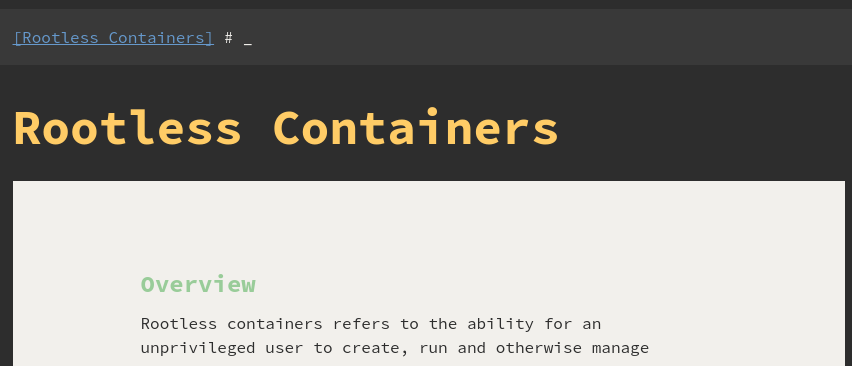
\includegraphics[width=\linewidth,height=0.6\textheight,keepaspectratio]{rootlesscontainers_website}
		    \caption{\tt\underline{rootlesscontaine.rs}}
		\end{figure}
	\end{frame}
	
	\begin{frame}{Kernel Stuff}
		\begin{itemize}
		    \item Currently only \texttt{btrfs} supports unprivileged ``subvolume'' operations.
		    \begin{itemize}
    		    \item Ubuntu ships \texttt{overlayfs} allowing unprivileged mounting.
		    \end{itemize}
		    \item The demo didn't create a new \texttt{NET} namespace --- it used the hosts's.
		    \begin{itemize}
		        \item \dots but what if we want to use cool networking and still have network access?
		        \item I have some horrific ideas with implementing \texttt{veth} in user-space.
		    \end{itemize}
		\end{itemize}
	\end{frame}

	\begin{frame}{Unprivileged clusters!}
		\begin{itemize}
			\item I have access to a bunch of nodes and want to manage jobs across those, what do I do?
			\item Biggest blocker looks to be networking (see \texttt{kube-proxy}).
			\item Most orchestrators assume root and it's hard to work around those assumptions upstream.
		\end{itemize}
	\end{frame}

	\begin{frame}[noframenumbering]{Unprivileged clusters!}
	    \begin{figure}
		    \centering
    		    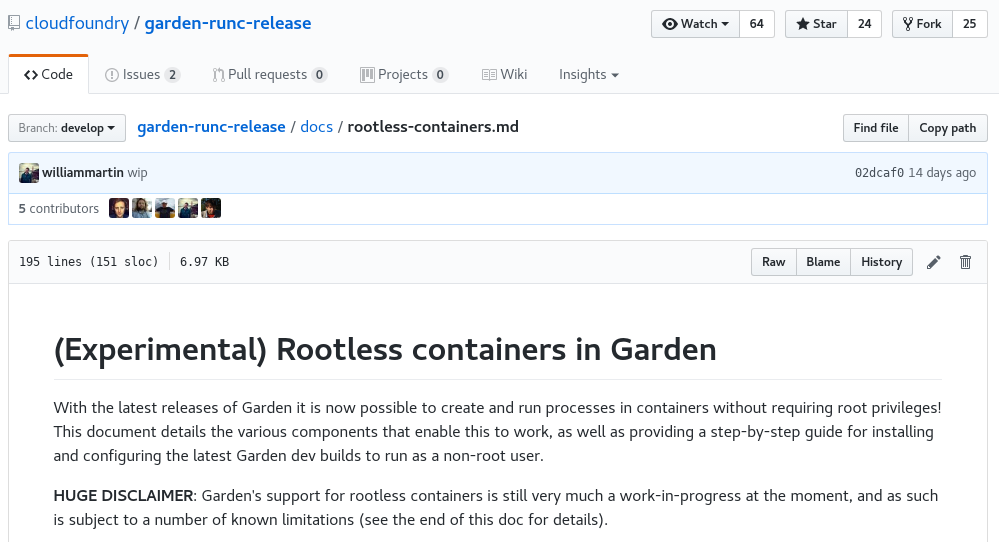
\includegraphics[width=\linewidth,height=0.6\textheight,keepaspectratio]{cf_screenshot}
	        \caption{\tt\underline{\url{https://github.com/cloudfoundry/garden-runc-release}}}
	    \end{figure}
	\end{frame}
	
	\begin{frame}{Contain absolutely everything!!}
		\begin{itemize}
		    \item Why stop at servers, why can't we run all of our things inside containers.
		    \item \href{https://github.com/flatpak/flatpak}{\tt\underline{Flatpak}} is working on this, but is not going all the way with containers.
		    \item If you can run it as your user, it should be able to work in rootless containers.
		    \begin{itemize}
		        \item \textit{Unprivileged overlay might have some interesting properties here~\dots}
		    \end{itemize}   
			\item \textit{Ultimate convergence \textsuperscript{TM}: What if you could use container features in desktop applications?}
		\end{itemize}
	\end{frame}


	\begin{frame}[noframenumbering]{Contain absolutely everything!!}
	    \begin{figure}
		    \centering
    		    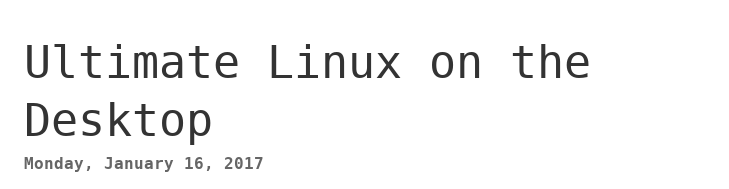
\includegraphics[width=\linewidth,height=0.6\textheight,keepaspectratio]{jessie_screenshot}
	        \caption{\tt\underline{\url{https://blog.jessfraz.com/post/ultimate-linux-on-the-desktop/}}}
	    \end{figure}
	\end{frame}

	\begin{frame}{Acknowledgements}
		\begin{itemize}
			\item \textbf{Jessie Frazelle} --- started working on this first and inspired me with her PoC, \href{https://github.com/jessfraz/binctr}{\underline{binctr}}.
			\item \textbf{Eric Biederman} and \textbf{Serge Hallyn} --- working tirelessly to get \texttt{USER} namespaces and countless other unprivileged kernel features working.
			\item \textbf{James Bottomley} --- helped me with kernel patches trying to fix the \texttt{cgroup} issue and also has done a lot of kernel ``container'' work.
		\end{itemize}
	\end{frame}

	\begin{frame}
		\begin{figure}
			{\Huge Questions?}
		    \caption{\small \underline{\url{https://www.cyphar.com/src/talks}}}
		\end{figure}
	\end{frame}
\end{document}